% ============================================================
\chapter{Transport Equation}
\label{ch:transport}
% ============================================================

Picture a river carrying a patch of dye downstream. No mixing, no diffusion---just pure displacement. The concentration profile glides along unchanged, as if riding an invisible conveyor belt. This deceptively simple scenario is the subject of the transport equation, the most elementary PDE one can write, yet one that already reveals the deep structure underlying all of partial differential equations.

The transport equation was studied as early as the eighteenth century by Euler and d'Alembert, who recognised that wave propagation and fluid flow both reduce, in their simplest form, to tracking quantities along characteristic curves. What makes this equation so instructive is that it can be solved exactly, by a geometric argument rather than an algebraic trick: one simply follows the flow. This method of characteristics, as we shall see, is the key that unlocks not only transport but a wide family of first-order PDEs.

\section{Introduction and physical motivation}

The transport equation is the simplest PDE. It models the displacement of
a quantity (concentration, density, pollutant) carried by a velocity field
without diffusion or reaction.

\begin{intuition}
Imagine dye injected into a river with a uniform current. The dye is carried
along without mixing: its concentration profile moves rigidly at the
current speed. This is exactly what the transport equation describes.
\end{intuition}

\section{Constant-coefficient transport equation}

\subsection{The Cauchy problem}

\begin{definition}[Homogeneous transport equation]
The \textbf{transport equation} with constant velocity $c \in \R$ is:
\begin{equation}\label{eq:transport_homogeneous}
    \begin{cases}
        u_t + c\, u_x = 0, & x \in \R,\; t > 0,\\
        u(x,0) = u_0(x), & x \in \R.
    \end{cases}
\end{equation}
\end{definition}

\begin{theorem}[Solution of the Cauchy problem]
If $u_0 \in C^1(\R)$, then problem \eqref{eq:transport_homogeneous}
admits a unique solution $u \in C^1(\R \times [0,+\infty))$ given by:
\begin{equation}\label{eq:transport_solution}
    \boxed{u(x,t) = u_0(x - ct).}
\end{equation}
\end{theorem}

\begin{proof}
\textbf{Method of characteristics.} We seek curves $(x(t), t)$ in the
$(x,t)$-plane along which the solution $u$ is constant. If $u$ is a
solution, set $z(t) = u(x(t), t)$. Then:
\[
    z'(t) = u_t(x(t),t) + x'(t)\, u_x(x(t),t).
\]
For $z'(t) = 0$ (constant along the curve), it suffices to choose
$x'(t) = c$, giving the \textbf{characteristics}:
\[
    x(t) = x_0 + ct, \quad x_0 \in \R.
\]
Along each characteristic, $u(x(t),t) = u(x_0, 0) = u_0(x_0)$.
Expressing $x_0 = x - ct$, we obtain $u(x,t) = u_0(x-ct)$.

\textbf{Verification.} If $u_0 \in C^1$, then $u(x,t) = u_0(x-ct)$
is $C^1$ and:
\[
    u_t = -c\, u_0'(x-ct), \quad u_x = u_0'(x-ct),
\]
so $u_t + c\, u_x = 0$ and $u(x,0) = u_0(x)$.

\textbf{Uniqueness.} If $v$ is another $C^1$ solution, then $w = u - v$
satisfies $w_t + c\, w_x = 0$ with $w(x,0) = 0$. Along every
characteristic, $w$ is constant equal to $0$, so $w \equiv 0$.
\end{proof}

\begin{center}
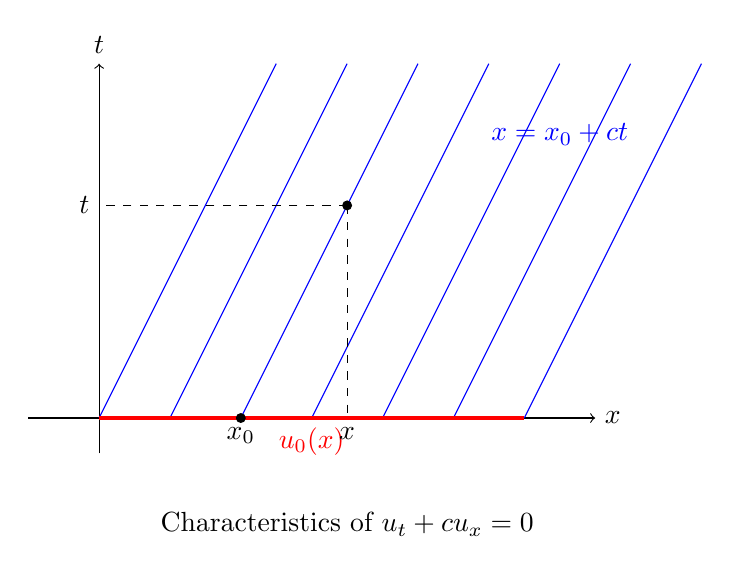
\begin{tikzpicture}[scale=0.9]
    \draw[->] (-1,0) -- (7,0) node[right] {$x$};
    \draw[->] (0,-0.5) -- (0,5) node[above] {$t$};
    % Characteristics
    \foreach \x in {0,1,2,3,4,5,6}{
        \draw[blue, thin] (\x,0) -- (\x+2.5, 5);
    }
    \node[blue] at (6.5, 4) {$x = x_0 + ct$};
    % Initial condition
    \draw[very thick, red] (0,0) -- (6,0);
    \node[red, below] at (3,0) {$u_0(x)$};
    % Point
    \fill (2,0) circle (2pt) node[below] {$x_0$};
    \fill (3.5,3) circle (2pt);
    \draw[dashed] (3.5,3) -- (3.5,0) node[below] {$x$};
    \draw[dashed] (3.5,3) -- (0,3) node[left] {$t$};
    \node at (3.5, -1.5) {Characteristics of $u_t + cu_x = 0$};
\end{tikzpicture}
\end{center}

\begin{keyformulas}[title=\textbf{Transport equation --- key formulas}]
\begin{itemize}
    \item Solution: $u(x,t) = u_0(x - ct)$ (travelling wave).
    \item Characteristics: lines $x - ct = \mathrm{const}$.
    \item The solution propagates at speed $c$ without distortion.
\end{itemize}
\end{keyformulas}

\subsection{Inhomogeneous equation}

\begin{theorem}[Transport with source term]
The problem:
\begin{equation}\label{eq:transport_source}
    \begin{cases}
        u_t + c\, u_x = f(x,t), & x \in \R,\; t > 0,\\
        u(x,0) = u_0(x),
    \end{cases}
\end{equation}
has solution:
\begin{equation}\label{eq:transport_source_sol}
    u(x,t) = u_0(x-ct) + \int_0^t f(x - c(t-s), s)\, ds.
\end{equation}
\end{theorem}

\begin{proof}
Along the characteristic $x(s) = x - c(t-s)$, we have:
\[
    \frac{d}{ds}u(x(s),s) = u_t + c\, u_x = f(x(s),s).
\]
Integrating from $s=0$ to $s=t$:
\[
    u(x,t) - u(x-ct, 0) = \int_0^t f(x - c(t-s), s)\, ds.
\]
\end{proof}

\section{Method of characteristics --- general case}

\subsection{First-order quasilinear PDEs}

Consider the general first-order PDE:
\begin{equation}\label{eq:quasilinear}
    a(x,y,u)\, u_x + b(x,y,u)\, u_y = c(x,y,u).
\end{equation}

\begin{definition}[Characteristic equations]
The \textbf{characteristic equations} associated with
\eqref{eq:quasilinear} form the ODE system:
\begin{equation}\label{eq:char_system}
    \frac{dx}{a(x,y,u)} = \frac{dy}{b(x,y,u)} = \frac{du}{c(x,y,u)}.
\end{equation}
Equivalently, parametrizing by $s$:
\[
    \frac{dx}{ds} = a, \quad \frac{dy}{ds} = b, \quad \frac{du}{ds} = c.
\]
\end{definition}

\begin{theorem}[Local existence]
Let $\Gamma$ be an initial curve parametrized by
$(x_0(\tau), y_0(\tau), u_0(\tau))$ such that:
\[
    \frac{\partial(x,y)}{\partial(s,\tau)}\bigg|_{s=0}
    = a\, y_0'(\tau) - b\, x_0'(\tau) \neq 0
    \quad \text{(transversality condition)}.
\]
Then there exists locally a unique solution $u(x,y)$ near $\Gamma$.
\end{theorem}

\begin{warning}[title=\textbf{Transversality condition}]
If the initial curve is tangent to the characteristics at a point, the
method fails: either there is no solution or infinitely many. This is
analogous to the Cauchy problem for ODEs when the initial condition is
posed at a singular point.
\end{warning}

\begin{example}[Linear PDE with variable coefficients]
Solve:
\[
    x\, u_x + y\, u_y = u, \quad u(x,1) = g(x).
\]
The characteristic equations are:
\[
    \frac{dx}{x} = \frac{dy}{y} = \frac{du}{u}.
\]
From $\frac{dx}{x} = \frac{dy}{y}$, we get $\frac{x}{y} = C_1$.
From $\frac{dy}{y} = \frac{du}{u}$, we get $\frac{u}{y} = C_2$.
So the general solution is:
\[
    u = y\, \Phi\!\left(\frac{x}{y}\right)
\]
for an arbitrary function $\Phi$. The initial condition $u(x,1) = g(x)$
gives $\Phi(x) = g(x)$, hence:
\[
    u(x,y) = y\, g\!\left(\frac{x}{y}\right).
\]
\end{example}

\subsection{Nonlinear case: Burgers' equation}

\begin{definition}[Inviscid Burgers' equation]
\textbf{Burgers' equation} is the nonlinear PDE:
\begin{equation}\label{eq:burgers}
    u_t + u\, u_x = 0, \quad u(x,0) = u_0(x).
\end{equation}
\end{definition}

\begin{theorem}[Implicit solution of Burgers' equation]
The characteristics of \eqref{eq:burgers} are the lines:
\[
    x = x_0 + u_0(x_0)\, t.
\]
Along each characteristic, $u$ is constant: $u = u_0(x_0)$.
The solution is defined implicitly by:
\begin{equation}\label{eq:burgers_implicit}
    u(x,t) = u_0(x - u(x,t)\, t).
\end{equation}
\end{theorem}

\begin{proof}
The characteristic equations are:
\[
    \frac{dx}{ds} = u, \quad \frac{dt}{ds} = 1, \quad \frac{du}{ds} = 0.
\]
So $u$ is constant along characteristics, and $x(t) = x_0 + u_0(x_0)\, t$.
\end{proof}

\subsection{Shock formation}

\begin{theorem}[Shock formation time]
If $u_0 \in C^1(\R)$ and $u_0'$ has a negative minimum, then the
characteristics cross at time:
\begin{equation}\label{eq:shock_time}
    t^* = \frac{-1}{\min_{x \in \R} u_0'(x)} > 0.
\end{equation}
For $t < t^*$, the solution is $C^1$. For $t \geq t^*$, a \textbf{shock}
(discontinuity) forms.
\end{theorem}

\begin{proof}
Two characteristics starting from $x_0$ and $x_1 > x_0$ cross if:
\[
    x_0 + u_0(x_0)\, t = x_1 + u_0(x_1)\, t,
\]
i.e., $t = \frac{x_1 - x_0}{u_0(x_0) - u_0(x_1)} = \frac{-1}{(u_0(x_1)-u_0(x_0))/(x_1-x_0)}$.
Taking $x_1 \to x_0$, the first crossing occurs at $t^* = -1/\min u_0'$.
\end{proof}

\begin{center}
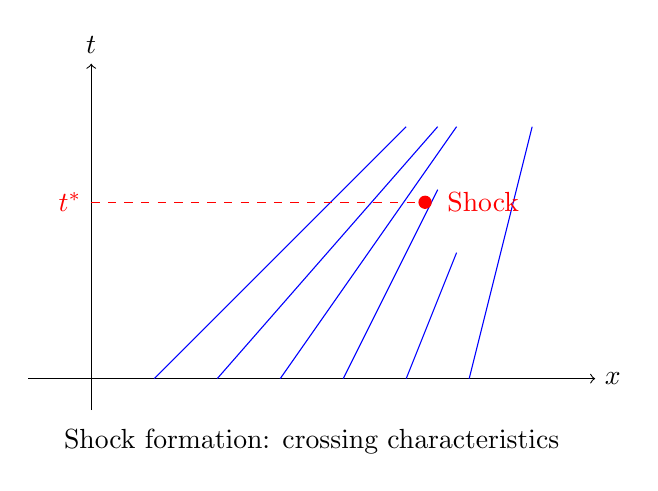
\begin{tikzpicture}[scale=0.8]
    \draw[->] (-1,0) -- (8,0) node[right] {$x$};
    \draw[->] (0,-0.5) -- (0,5) node[above] {$t$};
    % Crossing characteristics
    \draw[blue] (1,0) -- (5,4);
    \draw[blue] (2,0) -- (5.5,4);
    \draw[blue] (3,0) -- (5.8,4);
    \draw[blue] (4,0) -- (5.5,3);
    \draw[blue] (5,0) -- (5.8,2);
    \draw[blue] (6,0) -- (7, 4);
    % Crossing point
    \fill[red] (5.3, 2.8) circle (3pt);
    \node[red, right] at (5.5, 2.8) {Shock};
    % Critical time
    \draw[dashed, red] (0,2.8) -- (5.3,2.8);
    \node[red, left] at (0,2.8) {$t^*$};
    \node at (3.5, -1) {Shock formation: crossing characteristics};
\end{tikzpicture}
\end{center}

\begin{example}[Shock for Burgers' equation]
Let $u_0(x) = 1 - x$ for $x \in [0,1]$, $u_0(x) = 1$ for $x < 0$,
$u_0(x) = 0$ for $x > 1$. Then $\min u_0' = -1$ (on $(0,1)$), so
$t^* = 1$. The characteristics from $[0,1]$ are $x = x_0 + (1-x_0)t$
and they all meet at the point $(1,1)$.
\end{example}

\section{Transport in higher dimensions}

\begin{definition}[Transport equation in $\R^n$]
Let $\vec{b} = (b_1, \ldots, b_n) \in \R^n$ be a constant velocity vector.
The transport equation reads:
\begin{equation}\label{eq:transport_Rn}
    u_t + \vec{b} \cdot \nabla u = 0, \quad u(x,0) = u_0(x),
    \quad x \in \R^n.
\end{equation}
The solution is $u(x,t) = u_0(x - \vec{b}\, t)$.
\end{definition}

For a variable velocity field $\vec{b}(x,t)$, the equation
$u_t + \vec{b}(x,t) \cdot \nabla u = 0$ is still solved by
characteristics, which are solutions of:
\[
    \frac{d\vec{X}}{dt} = \vec{b}(\vec{X}(t), t), \quad \vec{X}(0) = x_0.
\]

\section{Conservation and first integrals}

\begin{proposition}[Conservation of $L^p$ norms]
If $u$ solves $u_t + c\, u_x = 0$ with $u_0 \in L^p(\R)$,
$1 \leq p \leq \infty$, then:
\[
    \norm{u(\cdot, t)}_{L^p(\R)} = \norm{u_0}_{L^p(\R)}
    \quad \forall t \geq 0.
\]
\end{proposition}

\begin{proof}
For $1 \leq p < \infty$, the change of variable $y = x - ct$ gives:
\[
    \int_\R \abs{u(x,t)}^p\, dx
    = \int_\R \abs{u_0(x-ct)}^p\, dx
    = \int_\R \abs{u_0(y)}^p\, dy.
\]
The case $p = \infty$ is immediate.
\end{proof}

\begin{theorem}[Conservative form and Rankine--Hugoniot condition]
The equation $u_t + (f(u))_x = 0$ (conservation law) admits discontinuous
weak solutions. Across a discontinuity propagating at speed $\sigma$,
the \textbf{Rankine--Hugoniot condition} reads:
\begin{equation}\label{eq:rankine_hugoniot}
    \sigma\, [u] = [f(u)],
\end{equation}
where $[u] = u^+ - u^-$ denotes the jump.
\end{theorem}

\section{Weak solutions and entropy}

\begin{definition}[Weak solution]
A function $u \in L^\infty(\R \times [0,\infty))$ is a \textbf{weak
solution} of $u_t + (f(u))_x = 0$ with initial data $u_0$ if:
\[
    \int_0^\infty \int_\R \bigl[u\, \varphi_t + f(u)\, \varphi_x\bigr]\, dx\, dt
    + \int_\R u_0(x)\, \varphi(x,0)\, dx = 0
\]
for all $\varphi \in C_c^\infty(\R \times [0,\infty))$.
\end{definition}

\begin{warning}[title=\textbf{Non-uniqueness of weak solutions}]
Weak solutions are generally not unique! One must impose an
\textbf{entropy condition} to select the physically admissible solution.
Lax's condition requires:
\[
    f'(u^-) > \sigma > f'(u^+).
\]
\end{warning}

\section{Exercises}

\begin{exercise}
Solve $u_t + 3u_x = 0$, $u(x,0) = e^{-x^2}$. Sketch $u(x,t)$ for
$t = 0, 1, 2$.
\end{exercise}

\begin{exercise}
Solve $u_t + 2u_x = t\sin x$, $u(x,0) = 0$.
\end{exercise}

\begin{exercise}
Solve by characteristics:
$y\, u_x - x\, u_y = 0$, $u(x,0) = x^2$ for $x > 0$.
Interpret the characteristics geometrically.
\end{exercise}

\begin{exercise}
Consider Burgers' equation $u_t + u\, u_x = 0$ with:
\[
    u_0(x) = \begin{cases}
        1 & \text{if } x < 0,\\
        1 - x & \text{if } 0 \leq x \leq 1,\\
        0 & \text{if } x > 1.
    \end{cases}
\]
\begin{enumerate}
    \item Draw the characteristics.
    \item Determine the shock formation time $t^*$.
    \item Write the solution for $0 < t < t^*$.
\end{enumerate}
\end{exercise}

\begin{exercise}
Solve the nonlinear transport equation:
$u_t + u^2 u_x = 0$, $u(x,0) = \frac{1}{1+x^2}$.
Determine the time of formation of the first shock.
\end{exercise}

\begin{exercise}
Show that if $u$ solves $u_t + c\, u_x = 0$, then
$E(t) = \frac{1}{2}\int_\R u^2(x,t)\, dx$ is conserved.
Generalize to $u_t + c(x)\, u_x = 0$ with $c_x = 0$.
What happens if $c_x \neq 0$?
\end{exercise}

\begin{exercise}[Rarefaction waves]
Consider Burgers' equation with:
\[
    u_0(x) = \begin{cases}
        0 & \text{if } x < 0,\\
        1 & \text{if } x > 0.
    \end{cases}
\]
\begin{enumerate}
    \item Show that no classical solution exists for $t > 0$.
    \item Construct a \textbf{rarefaction wave} $u(x,t) = v(x/t)$ that
          is a continuous weak solution.
    \item Verify that a shock solution (with speed $\sigma = 1/2$) is
          also a weak solution, but does not satisfy Lax's entropy
          condition.
\end{enumerate}
\end{exercise}
